\documentclass[12pt, a4paper, oneside, UTF8]{ctexart}
\usepackage{amsmath, amsthm, amssymb, bm, color, framed, graphicx, hyperref, mathrsfs}
\usepackage{geometry}
\geometry{left = 2.5 cm, right = 2.5 cm, top = 2.5 cm, bottom = 2.5 cm}

\title{\textbf{作业5}\\{\small (数值算法与案例分析)}}
\author{李维杰}
\date{\today}
\linespread{1.5}
\definecolor{shadecolor}{RGB}{241, 241, 255}
\newcounter{problemname}
\newenvironment{problem}{\begin{shaded}\stepcounter{problemname}\par\noindent\textbf{题目\arabic{problemname}. }}{\end{shaded}\par}
\newenvironment{solution}{\par\noindent\textbf{解答. }}{\par}
\newenvironment{note}{\par\noindent\textbf{注记. }}{\par}

\begin{document}

\maketitle

\begin{problem}
    设矩阵$A\in{\mathbb{C}^{{m}\times{n}}}({m}\geq{n})$.编写程序,分别使用CGS,MGS,CGS2,MGS2算法求矩阵$A$的$QR$分解,并通过一些例子可视化正交性损失${\left\lVert{Q^*Q-I_n}\right\rVert}_{\mathsf{F}}$.
\end{problem}

\begin{solution}
    \begin{figure}[htbp] % 创建一个图形环境
        \centering % 图片居中
        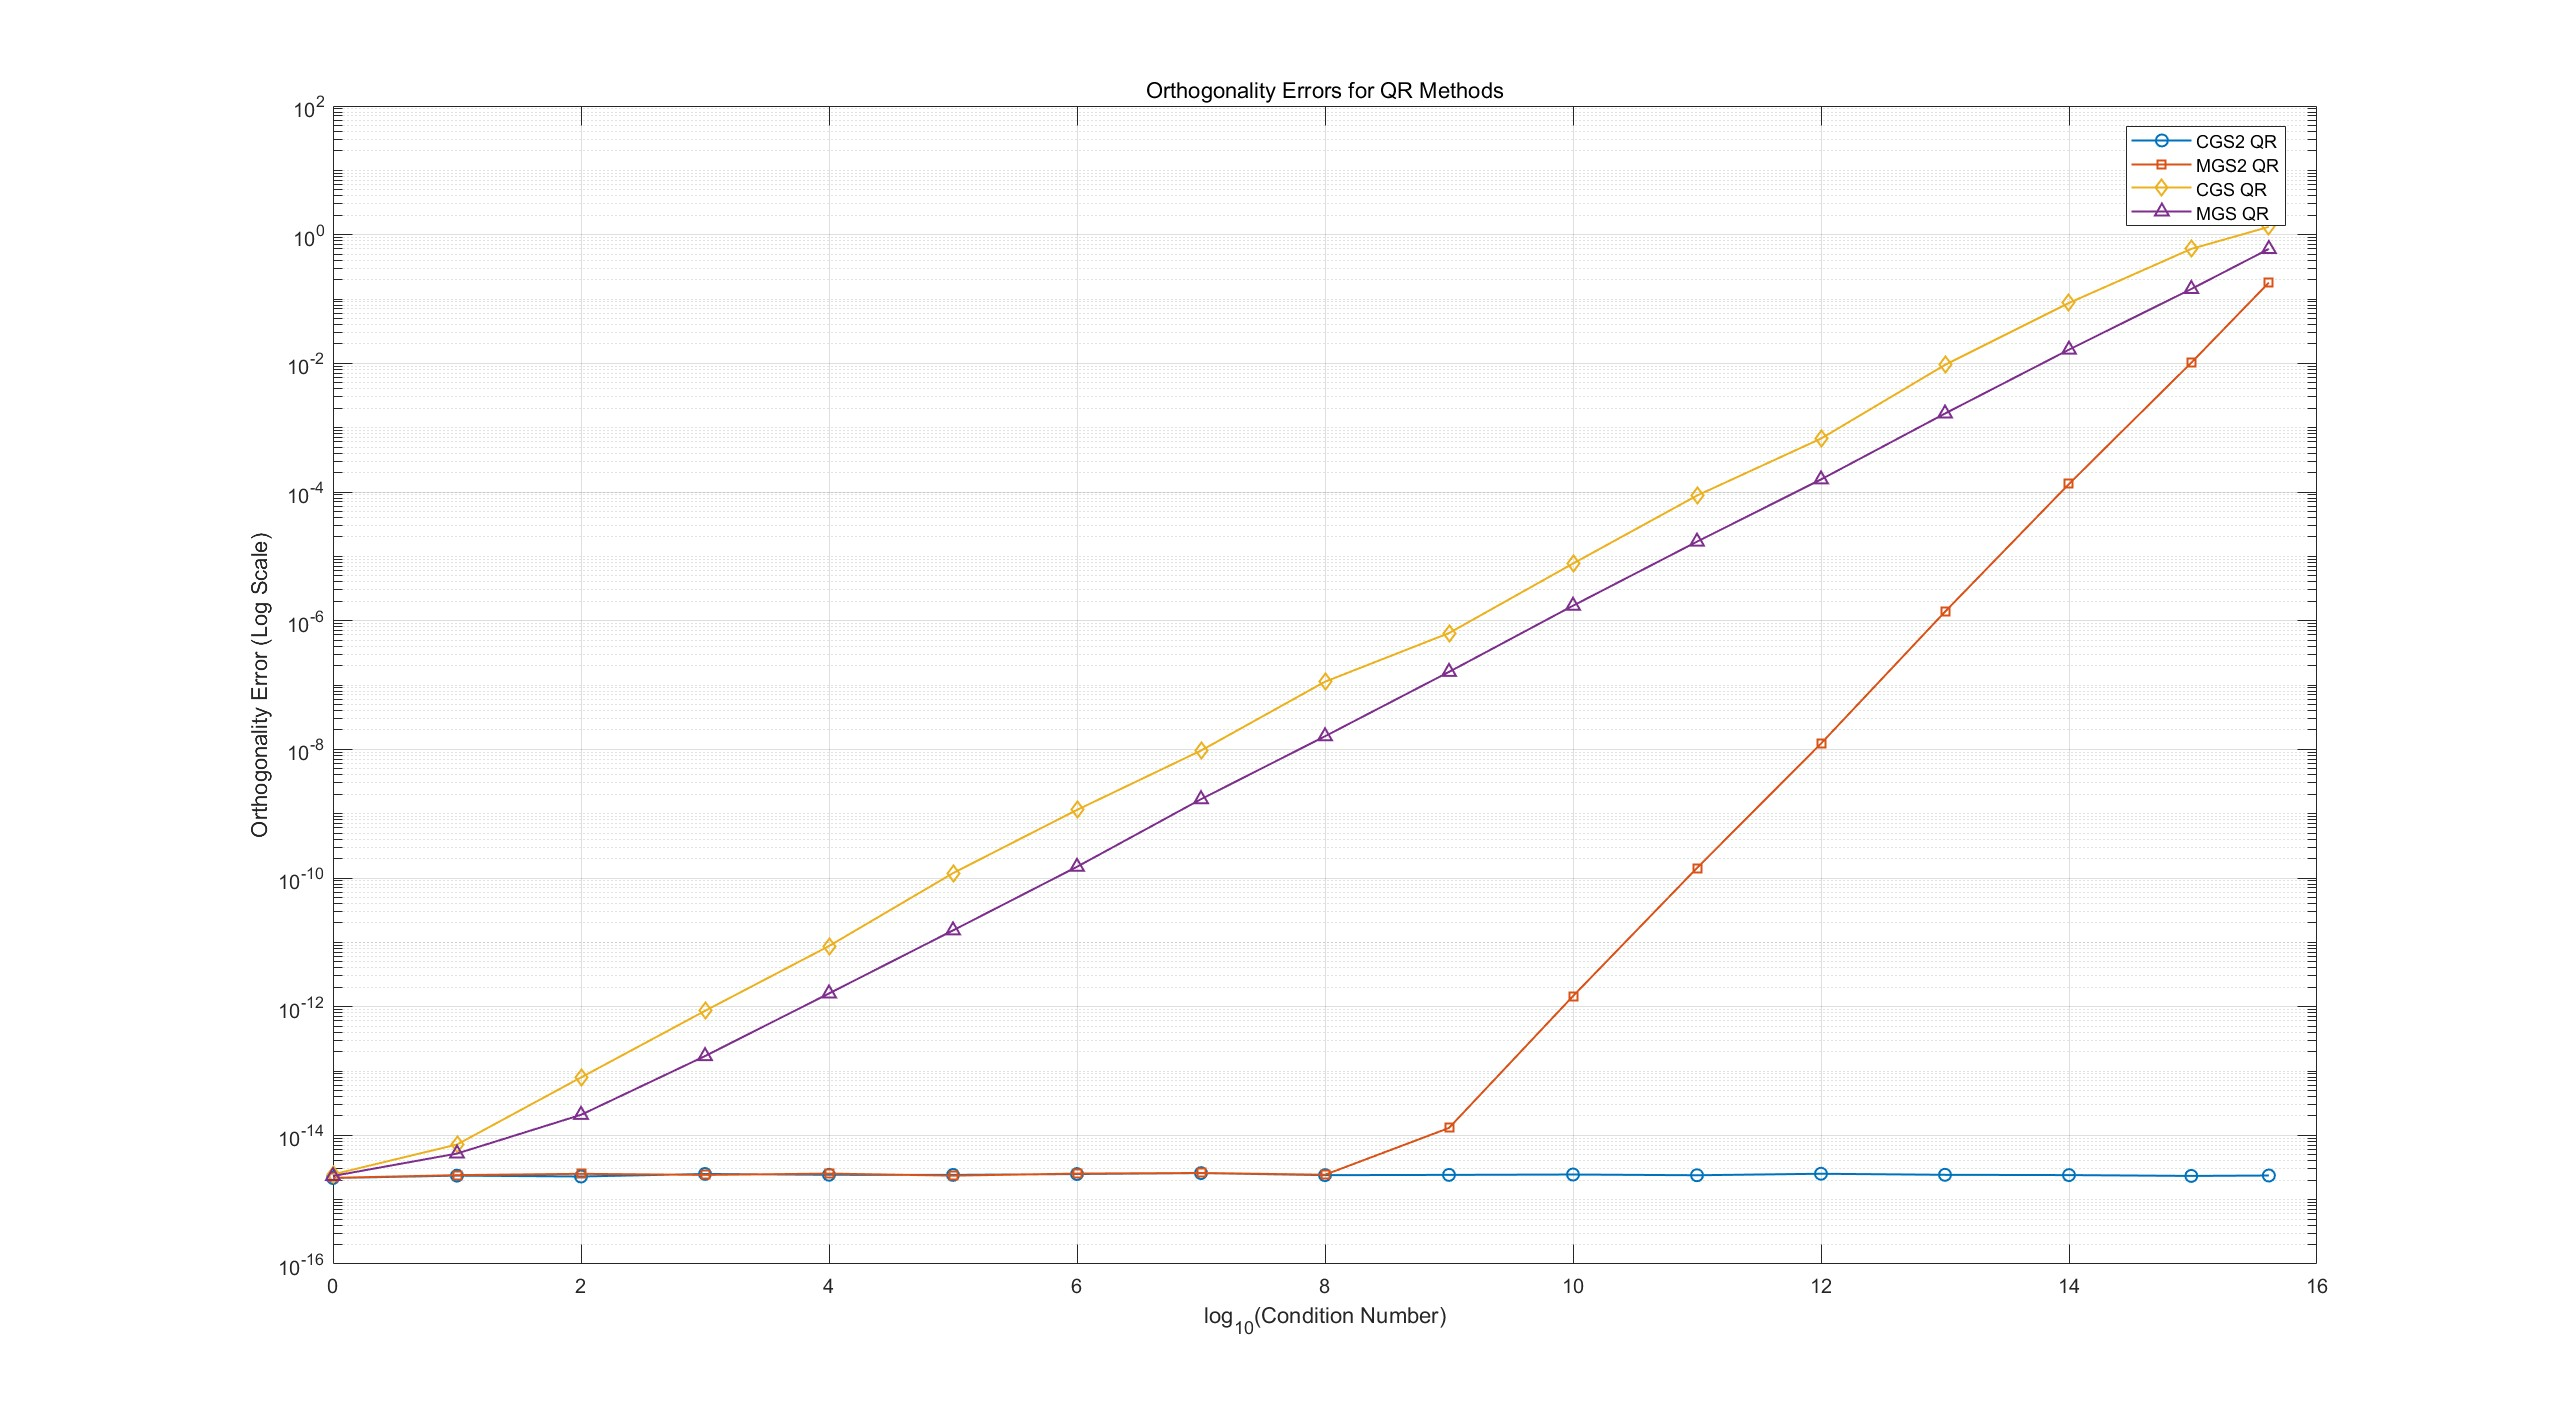
\includegraphics[scale=0.17]{Problem1.jpg} % 插入图片,设置宽度为页面宽度的70%
        \caption{${\left\lVert{Q^*Q-I_n}\right\rVert}_{\mathsf{F}}$与$\lg{\kappa(A)}$的关系曲线图} % 图片的说明文字
    \end{figure}
\end{solution}

\begin{note}
    暂不清楚为什么我的代码跑出来的MGS2在条件数较大时数值稳定性会变差.debug未果...
\end{note}

\begin{problem}
    生成一些满足$\kappa\in[10^{0},10^{15}]$的瘦高矩阵,并可视化Householder-QR,Cholesky-QR,CGS,MGS这四种算法下的正交性损失${\left\lVert{Q^*Q-I_n}\right\rVert}_{\mathsf{F}}$和剩余范数${\left\lVert{A-QR}\right\rVert}_{\mathsf{F}}$.
\end{problem}

\begin{solution}
    \begin{figure}[htbp] % 创建一个图形环境
        \centering % 图片居中
        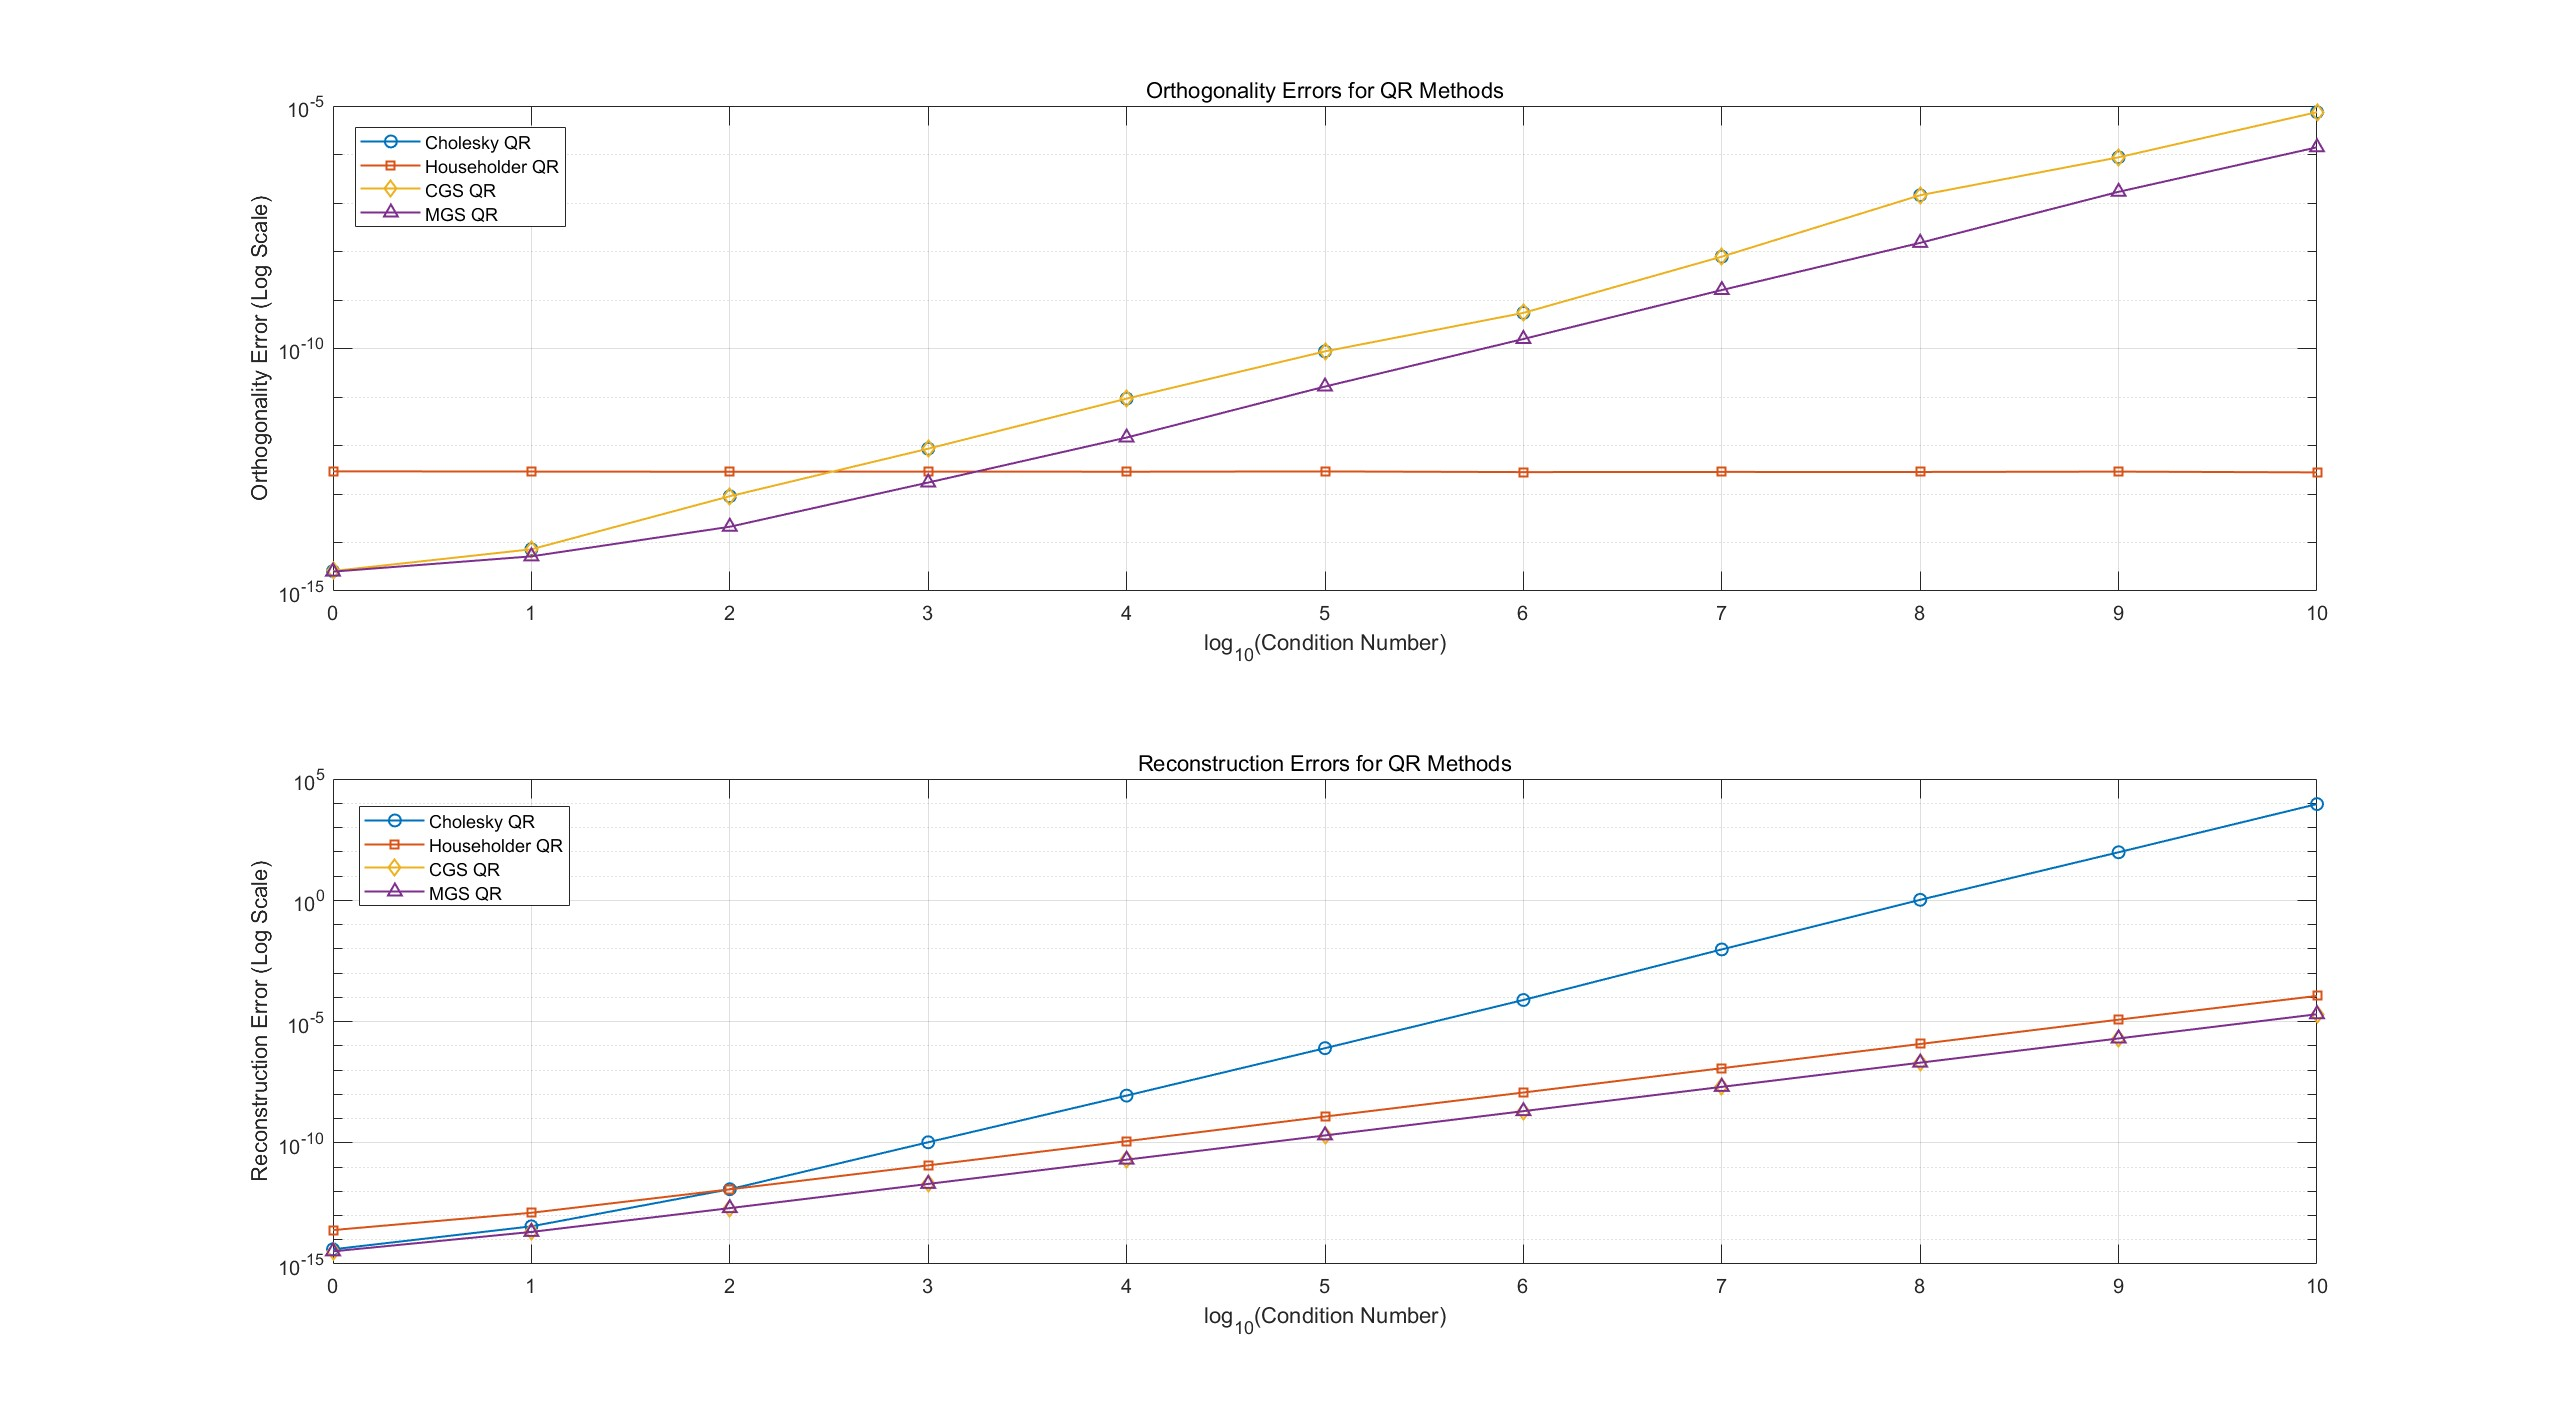
\includegraphics[scale=0.17]{Problem2.jpg} % 插入图片,设置宽度为页面宽度的70%
        \caption{${\left\lVert{Q^*Q-I_n}\right\rVert}_{\mathsf{F}}$和${\left\lVert{A-QR}\right\rVert}_{\mathsf{F}}$与$\lg{\kappa(A)}$的关系曲线图} % 图片的说明文字
    \end{figure}
\end{solution}

\begin{problem}
    设$A\in{\mathbb{C}^{{m}\times{n}}}$.证明:$AA^{\dagger}$和$I_n-A^{\dagger}A$分别是$\text{Range}(A)$和$\text{Ker}(A)$的正交投影.
\end{problem}

\begin{solution}
    由于
    \begin{align*}
        (AA^{\dagger})^2=A(A^*A)^{-1}A^*A(A^*A)^{-1}A^*=A(A^*A)^{-1}A^*=AA^{\dagger},
    \end{align*}
    故$AA^{\dagger}$是一个幂等矩阵,即其是一个投影矩阵.
    另外,由于
    \begin{align*}
        (AA^{\dagger})^*=(A(A^*A)^{-1}A^*)^*=A(A^*A)^{-1}A^*=AA^{\dagger},
    \end{align*}
    故此时有
    \begin{align*}
        <AA^{\dagger}x,(I-AA^{\dagger})x>&=(AA^{\dagger})^*(I-AA^{\dagger})\\
        &=(AA^{\dagger})^*-(AA^{\dagger})^*AA^{\dagger}\\
        &=AA^{\dagger}-(AA^{\dagger})^2\\
        &=0,
    \end{align*}
    即$AA^{\dagger}$是一个正交投影阵.
    进一步地,对于$\text{Range}(A)$中的任意向量$Ax$,均有
    \begin{align*}
        AA^{\dagger}Ax=A(A^*A)^{-1}A^*Ax=Ax,
    \end{align*}
    故可知$AA^{\dagger}$是作用于$\text{Range}(A)$上的正交投影阵.\\
    另一方面,$(I-AA^{\dagger})x$是$AA^{\dagger}x$的正交分量,且$\text{Ker}(A)\bot\text{Range}(A)$,
    于是可以直接得到$I-AA^{\dagger}$是作用于$\text{Ker}(A)$上的正交投影阵.
\end{solution}

\begin{problem}
    设$A\in{\mathbb{C}^{{m}\times{n}}},X\in{\mathbb{C}^{{n}\times{m}}}$.假设对于任意的$b\in{\mathbb{C}^{m}}$,$x=Xb$总是最小二乘问题$\min_{x}{\left\lVert{Ax-b}\right\rVert}_{2}$的极小值点.证明$AXA=A$,且$(AX)^*=AX$.
\end{problem}

\begin{solution}
    作为最小二乘问题$\min_{x}{\left\lVert{Ax-b}\right\rVert}_{2}$的极小值点,$x$应满足
    \begin{align*}
        A^*Ax=A^*b,
    \end{align*}
    代入$x=Xb$,即得
    \begin{align*}
        A^*AXb=A^*b.
    \end{align*}
    由于$b$是任意的$m$维向量,故上式始终成立当且仅当
    \begin{align}
        A^*AX=A^*.
    \end{align}
    对(1)式左乘$X^*$,得
    \begin{align*}
        (AX)^*AX=(AX)^*.
    \end{align*}
    对(1)式两边同时取转置,得
    \begin{align*}
        (AX)^*A=A\Rightarrow(AX)^*AX=AX.
    \end{align*}
    综合以上二式,即得
    \begin{align*}
        (AX)^*=AX.
    \end{align*}
    从而得到
    \begin{align*}
        (AX)^*A=A\Rightarrow{AXA=A}.
    \end{align*}
\end{solution}

\begin{problem}
    找出针对数据集$\{(n,\ln{n})\in{\mathbb{R}^{2}}:n\in\{2,3,4,5,6,7\}\}$最好的拟合直线.可视化这一结果并解释拟合最优的原因.
\end{problem}

\begin{solution}
    设拟合直线为$\hat{y}=kx+t$,实际值为$y=\ln{x}$.又设
    \begin{align*}
        A =
        \left[
            \begin{array}{cccccc}	
                2 & 1 \\
                3 & 4 \\
                4 & 1 \\
                5 & 1 \\
                6 & 1 \\
                7 & 1
            \end{array}
        \right],
        x =
        \left[
            \begin{array}{cc}	
                k \\
                t \\
            \end{array}
        \right],
        y = 
        \left[
            \begin{array}{cccccc}	
                \ln{2} \\
                \ln{3} \\
                \ln{4} \\
                \ln{5} \\
                \ln{6} \\
                \ln{7}
            \end{array}
        \right],
    \end{align*}
    则只需找到合适的$x$,使得${\left\lVert{Ax-y}\right\rVert}_{2}$最小化即可.极小值点为
    \begin{align*}
        x=A^{\dagger}y=\left[
            \begin{array}{cc}	
                0.245 \\
                0.319 \\
            \end{array}
        \right].
    \end{align*}
    利用Matlab计算拟合直线并制图如下
    \begin{figure}[htbp] % 创建一个图形环境
        \centering % 图片居中
        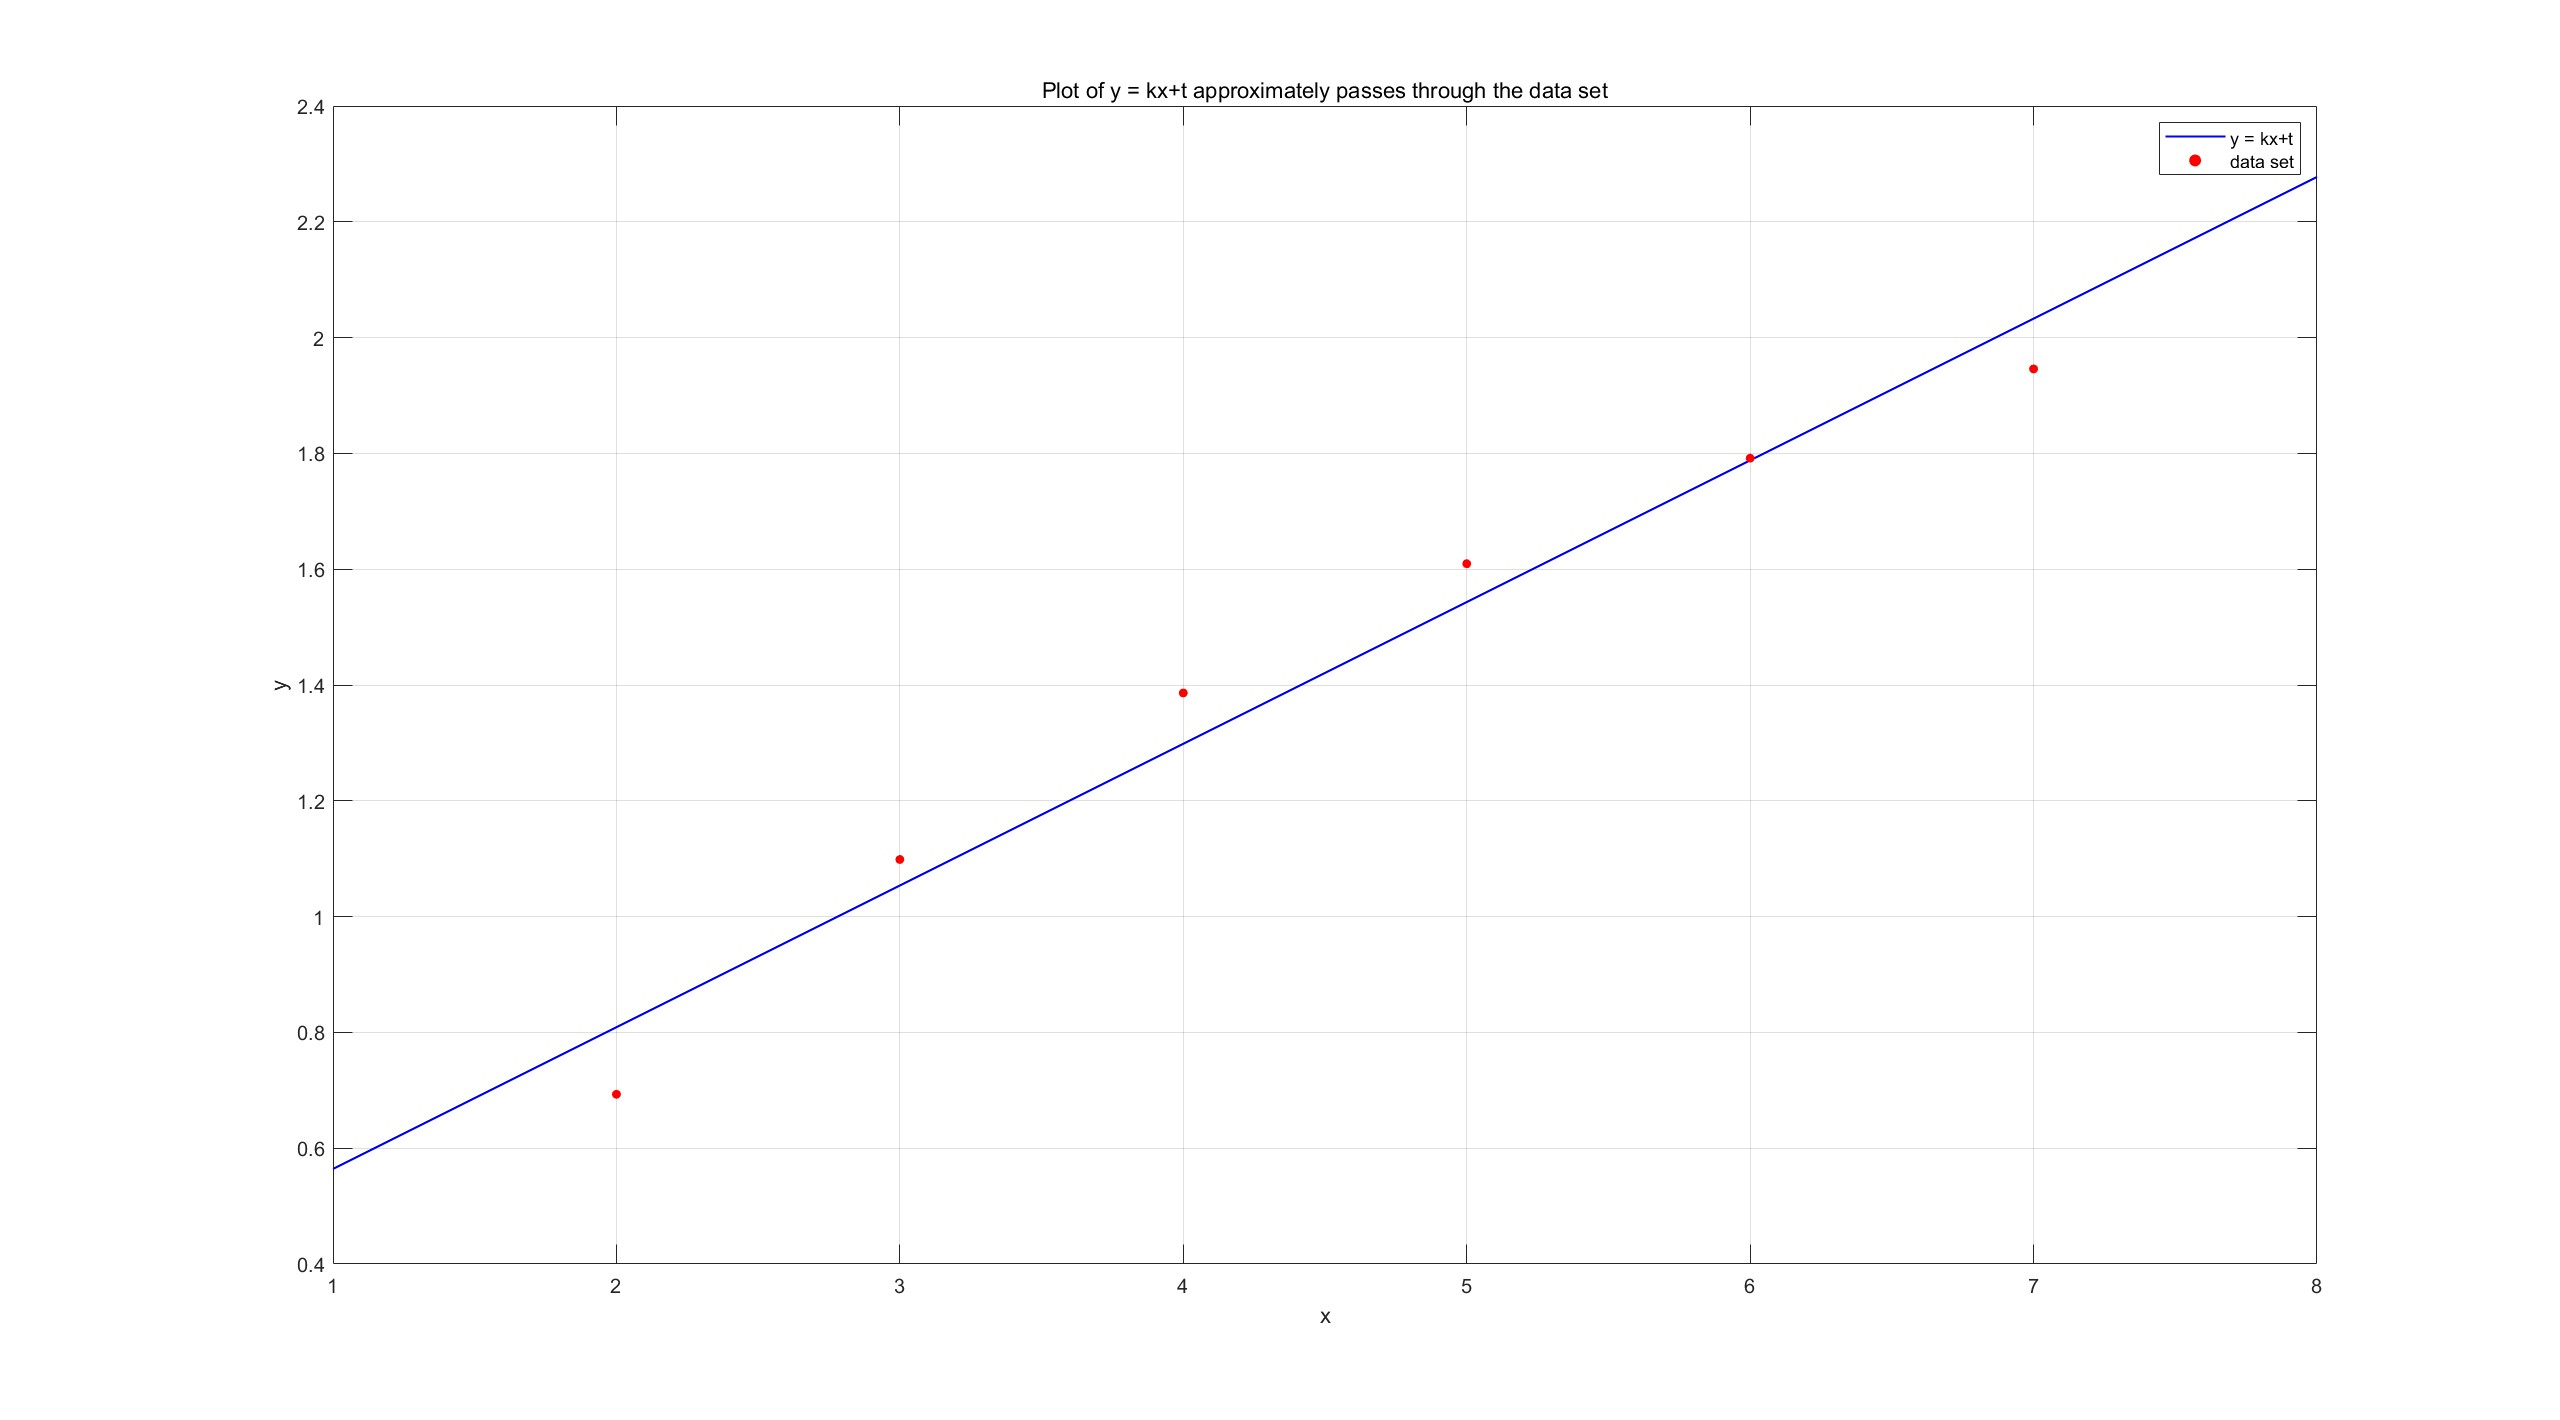
\includegraphics[scale=0.17]{Problem5.jpg} % 插入图片,设置宽度为页面宽度的70%
        \caption{数据集的拟合直线} % 图片的说明文字
    \end{figure}
\end{solution}
\end{document}